\section{数据与实验设计}
\label{sec:data}

\subsection{研究设计与证据图}
\label{subsec:data_sources}

经验分析覆盖华盛顿特区、纽约市和温哥华，时间范围为 2020 年 1 月 1 日至
2022 年 12 月 31 日。选择这三个城市，是因为它们在共同研究期内均提供
带地理坐标的案件记录和大规模公共自行车系统档案。犯罪记录分别来自
华盛顿特区警察局、纽约市警察局和温哥华警察局开放数据门户
\citep{dc_crime_data,nypd_crime_data,vpd_crime_data}；自行车行程分别
来自 Capital Bikeshare、Citi Bike 和 Mobi by Rogers
\citep{capital_bikeshare_data,citibike_data,mobi_data}。

图~\ref{fig:problem_chain} 把三个研究问题与所需证据相连接，图
\ref{fig:analysis_workflow} 则概括经验分析流程。犯罪和自行车记录首先
在事件层面标准化，随后聚合为共同 1~km 网格上的完整日面板。上支路估计
条件熵、条件互信息（CMI）和精确 DELB；下支路评估匹配的整数值预测器。
只有在信息集与评估期完全对齐后，才合并两条支路的输出。

\begin{figure}[H]
\centering
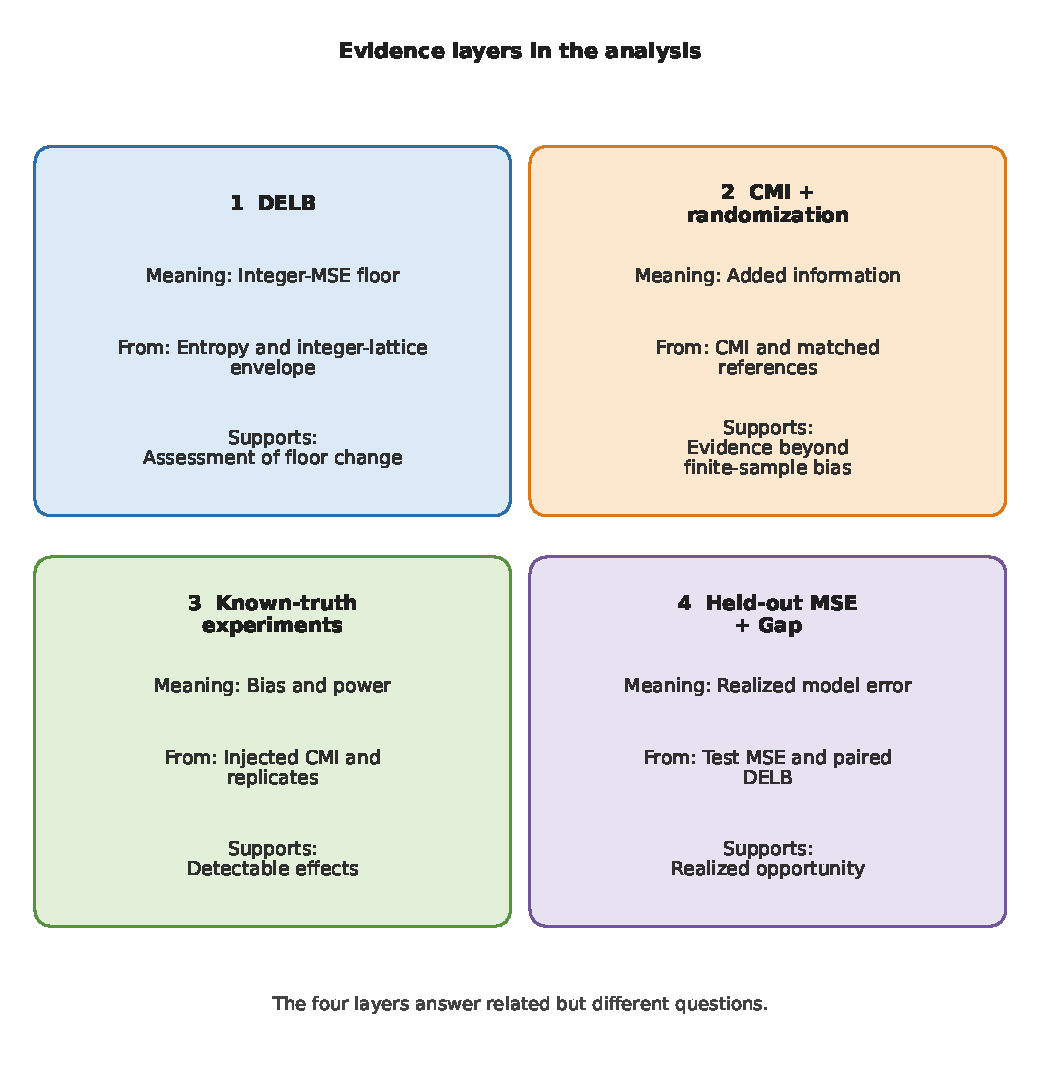
\includegraphics[width=\textwidth]{figures/problem_chain/unified_problem_chain.pdf}
\caption{统一问题链。总体 DELB 与 CMI 定义信息论误差底线，有限样本层区分点估计、
估计量偏差和随机化参考，城市应用再把校准证据与实际预测误差连接。该图由独立
Python 程序生成。}
\label{fig:problem_chain}
\end{figure}

\begin{figure}[H]
\centering
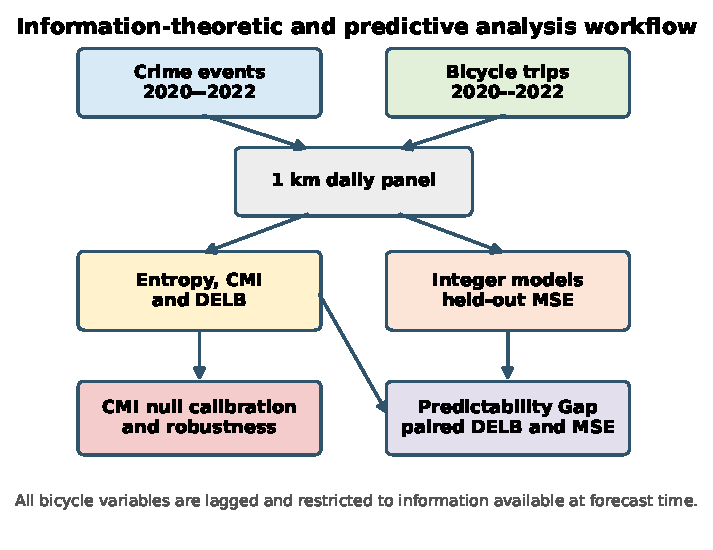
\includegraphics[width=\textwidth]{figures/e11/e11_analysis_workflow.pdf}
\caption{Information-theoretic and predictive analysis workflow. All
bicycle variables are lagged and restricted to information observed when
the one-day-ahead forecast is issued.}
\label{fig:analysis_workflow}
\end{figure}

\subsection{犯罪事件与跨城市统一}
\label{subsec:crime_data}

原始犯罪文件在事件层面进行统一。我们直接保留权威标准字段
\texttt{crime\_type\_\allowbreak unified}，后续实验不再重新分类。分析目标合并三个
互斥类别：财产盗窃、机动车盗窃和入室盗窃。源类别对照表见
附录~\ref{app:empirical_details}。事件按照源文件日历年份归属；华盛顿特区
35 条事件日期不在源文件年份内的记录被写入带原因编码的排除表。
为保证可审计性，保留稳定事件 ID、源文件哈希、源行号、原始类别、
时间戳和坐标。

清洗后得到 503,157 条有效犯罪事件。应用下述预先规定的空间范围后，
\TotalCrimeEvents{} 条事件进入完整分析面板。主要预测目标
\(C_{c,i,t}\) 是城市 \(c\)、网格 \(i\)、当地日期 \(t\) 上三个统一
类别的未分箱日计数。分类别计数仅用于异质性分析。

\subsection{自行车行程与端点流量}
\label{subsec:bicycle_data}

三个自行车系统的字段模式随时间变化。数据处理将其标准化为共同行程接口，
包括起止时间、站点 ID、站点名称、端点坐标、坐标来源、源标识符和
质量控制标记。输入文件采用分块处理，月份归属由行程开始时间决定。
空行和属于其他源月份的行程进入带原因编码的排除表。正式 ride ID 在
确定性保留首条记录后必须唯一。温哥华缺少正式唯一 ride ID 的完全重复
记录予以保留并标记，而不是静默删除。

有效时优先使用源坐标。华盛顿特区和纽约缺失坐标由稳健站点--月份中位数
及时间相邻观测恢复。温哥华端点先按官方站点 ID 匹配，再按所提供官方
站点文件中的唯一规范化站名匹配。workshop、service、testing、yard、
storage、production、temporary 和 valet 节点被标记为非公共节点。
无法解析的端点保留在标准化行程表中，但该端点不具备空间流量资格；
若另一端点已解析且为公共端点，则仍可贡献流量。

对每个网格--日期，出发与到达量定义
\(B^{\mathrm{out}}_{c,i,t}\) 和 \(B^{\mathrm{in}}_{c,i,t}\)，
总端点流量为
\[
B^{\mathrm{total}}_{c,i,t}
=B^{\mathrm{out}}_{c,i,t}+B^{\mathrm{in}}_{c,i,t}.
\]
主要移动变量是总流量的一日滞后。它在不把确定性冗余的总流量、净流量、
流入和流出同时放入同一熵状态的前提下，统计行程两端可观测活动。
共保留 87,208,600 条标准化行程，其中 \TotalBicycleTrips{} 条至少有
一个端点在分析网格中且具备流量资格。

\subsection{空间与时间面板构建}
\label{subsec:panel_construction}

坐标在各城市适当的坐标参考系中投影，并分配到以投影坐标系原点为锚点的
确定性 1~km 方格。城市层面点估计预先规定两个由训练期冻结的总体。完整
犯罪支持域包括 2020--2021 年至少发生过一件犯罪的所有网格；自行车覆盖域
是其中训练期自行车总流量为正的子集。两者均不使用任何 2022 年记录。
完整犯罪支持域之外的自行车端点仍保留在对账输出中，但不进入任一分析总体。

每个保留网格与全部 1096 个日历日交叉，包括零犯罪和零流量日期。完整面板
覆盖 1133 个网格，共有 \TotalPanelRows{} 条网格--日观测。自行车覆盖面板
是该完整面板的固定空间子集，而不是按非零流量日期重新构造。只有在构造
滞后分析时，每个网格的第一天才被移除。

时间切分在模型估计前固定：2020--2021 年用于训练，2022 年 1--6 月用于
验证，2022 年 7--12 月用于测试。空间资格、自行车覆盖状态和自行车离散化
阈值仅由训练期记录确定；模型超参数只使用训练与验证数据选择。测试期不参与
定义分析域、阈值、模型设定或纳入资格。预测所用变量在预测发出时均已可得，
信息集中不含同期或未来犯罪与移动记录。表~\ref{tab:variable_availability}
明确列出变量时序，表~\ref{tab:descriptive_statistics} 汇总完整面板。

\begin{table}[!htbp]
\caption{变量、分析单位及预测时可用性。“是，滞后”表示一步超前预测仅使用上一
聚合期的信息。}
\label{tab:variable_availability}
\centering
\footnotesize
\begin{tabularx}{\textwidth}{p{2.3cm}Xp{1.9cm}p{1.9cm}p{2.2cm}}
\toprule
\textbf{变量} & \textbf{含义与作用} & \textbf{空间单位} &
\textbf{时间单位} & \textbf{预测时可用}\\
\midrule
犯罪计数 & 三类统一犯罪的每日事件数；未分箱预测目标 & 1 km 网格 & 日 &
目标，否\\
滞后犯罪 & 上一时期犯罪计数，离散为 \(\{0,1,2,\geq3\}\)；基准状态 &
1 km 网格 & 前一日 & 是，滞后\\
自行车流入 & 已解析公共端点的到达数；移动原始量 & 1 km 网格 & 前一日 &
是，滞后\\
自行车流出 & 已解析公共端点的出发数；移动原始量 & 1 km 网格 & 前一日 &
是，滞后\\
自行车总流量 & 流入与流出之和，按训练期阈值离散；新增数据状态 &
1 km 网格 & 前一日 & 是，滞后\\
日历状态 & 星期、气象季节和公共假日状态；基准状态 & 城市/网格 & 预测日 &
是\\
网格标识 & 验证与测试前固定的空间状态；基准状态 & 1 km 网格 & 固定 & 是\\
\bottomrule
\end{tabularx}
\end{table}


\begin{table}[H]
\caption{Descriptive statistics for the complete 1 km grid--day panels, 2020--2022.}
\label{tab:descriptive_statistics}
\begin{adjustwidth}{-\extralength}{0cm}
\centering
\begin{tabular}{lrrrrrrr}
\toprule
\textbf{City} & \textbf{Grids} & \textbf{Grid--days} &
\textbf{Crime events} & \textbf{Bike trips} &
\textbf{Mean crime} & \textbf{Mean bike flow} & \textbf{Zero crime}\\
\midrule
Washington, DC & 186 & 203,856 & 71,397 & 7,620,562 & 0.350 & 72.95 & 77.0\%\\
New York City & 806 & 883,376 & 359,284 & 76,418,121 & 0.407 & 172.82 & 79.7\%\\
Vancouver & 141 & 154,536 & 72,447 & 2,231,293 & 0.469 & 27.37 & 75.3\%\\
\bottomrule
\end{tabular}
\end{adjustwidth}
\end{table}


在网格--日尺度上，犯罪计数高度稀疏，零计数占 75.3--79.7\%。
纽约的系统规模最大且平均自行车端点流量最高；温哥华的平均网格--日
财产犯罪计数最高。因此，本文报告城市特定结果，而不将合并记录视为可交换。

\subsection{描述性分析}
\label{subsec:descriptive_analysis}

熵估计前计算月度和空间汇总。犯罪与自行车流量的月度 Spearman
相关系数在华盛顿特区、纽约和温哥华分别为 0.505、0.603 和 0.221。
网格三年总量的对应相关系数分别为 0.637、0.651 和 0.633。
犯罪总量最高的前 10\% 网格分别集中了 43.9\%、54.3\% 和 54.1\%
的犯罪，却集中了 67.5\%、89.0\% 和 79.7\% 的自行车流量。
这些仅为描述性关联，尚未控制犯罪历史或日历状态。

相应的空间集中度和月度序列图移至独立补充材料第 S6 节，使正文直接进入 DELB
估计对象及其有限样本验证。

\subsection{评价设计概述}
\label{sec:methods}

证据按研究问题顺序解释。在定义目标和信息集后，依次检查 DELB 数值实现，
用已知真值模拟和支持度诊断刻画 CMI 的有限样本行为，估计城市与局部点值，
以三种随机化参考校准，最后比较匹配的留出预测。Fano、犯罪类别与替代设定
属于次要检查。

\subsection{目标与操作化信息集}
\label{subsec:operational_information_sets}
\label{subsec:methods_information_sets}

在应用中，第~\ref{sec:theory} 节的一般目标映射为
\begin{equation}
X_t\longmapsto C_{c,i,t}\in\mathbb Z_{\geq0},
\label{eq:crime_count_definition}
\end{equation}
即城市 \(c\)、网格 \(i\)、日期 \(t\) 的未分箱计数。自行车出发与到达定义为
\begin{equation}
B^{\mathrm{out}}_{c,i,t}
=\text{departures from }(c,i,t),
\qquad
B^{\mathrm{in}}_{c,i,t}
=\text{arrivals at }(c,i,t),
\label{eq:bicycle_in_out}
\end{equation}
原始向量为
\begin{equation}
\mathbf B_{c,i,t}
=
(B^{\mathrm{out}}_{c,i,t},B^{\mathrm{in}}_{c,i,t})^\top,
\label{eq:bicycle_primitive_vector}
\end{equation}
总流量、净流量和滞后块分别为
\begin{align}
B^{\mathrm{total}}_{c,i,t}
&=B^{\mathrm{out}}_{c,i,t}+B^{\mathrm{in}}_{c,i,t},
\label{eq:bicycle_total_flow}\\
B^{\mathrm{net}}_{c,i,t}
&=B^{\mathrm{in}}_{c,i,t}-B^{\mathrm{out}}_{c,i,t},
\label{eq:bicycle_net_flow}
\end{align}
\begin{equation}
\mathbf B^{(q)}_{c,i,t}
=
(\mathbf B_{c,i,t-1},\ldots,\mathbf B_{c,i,t-q}).
\label{eq:bicycle_lag_block}
\end{equation}
总流量和净流量是原始向量的确定性函数，不在同一熵状态中冗余加入。

上述理论对象被操作化为提前一天预测。目标始终是原始
非负整数计数，只有条件变量被离散化。前一日犯罪计数映射为
\(\{0,1,2,\geq3\}\)。在每个城市内，滞后总自行车流量的正值按照训练期
三分位切分，零流量单独构成一个状态。因此，自行车状态属于
\(\{\text{zero},\text{low},\text{medium},\text{high}\}\)，估计切点在
验证期和测试期保持不变。

基线信息状态为
\begin{equation}
\mathcal{S}^{0}_{c,i,t}
=\left(i,Q_C(C_{c,i,t-1}),d_t,s_t,h_t\right),
\label{eq:empirical_baseline_state}
\end{equation}
其中 \(d_t\)、\(s_t\) 和 \(h_t\) 分别表示星期、气象季节和公共假日状态。
移动增强状态为
\begin{equation}
\mathcal{S}^{B}_{c,i,t}
=\left(\mathcal{S}^{0}_{c,i,t},
Q_B(B^{\mathrm{total}}_{c,i,t-1})\right).
\label{eq:empirical_bicycle_state}
\end{equation}
该匹配状态设计在两个信息集之间只改变一个成分，即滞后自行车流量，并排除
同期或未来移动信息。以 sigma 代数表示，
\begin{align}
\mathcal F^0_{c,i,t}
&=\sigma(\mathcal S^0_{c,i,t}),
\label{eq:baseline_information}\\
\mathcal F^B_{c,i,t}
&=\mathcal F^0_{c,i,t}\vee
\sigma\{Q_B(\mathbf B^{(q)}_{c,i,t})\}.
\label{eq:bike_information}
\end{align}
已报告的主要分析未使用天气和土地利用协变量，因此本文不把
它们表述为已控制变量。

\subsection{犯罪计数与自行车信息的专门化}
\label{subsec:theory_application_appendix}

使用上述变量，基准熵与下界为
\begin{align}
H^0_{c,i,t}
&=H(C_{c,i,t}\mid\mathcal F^0_{c,i,t}),
\label{eq:crime_baseline_entropy}\\
L^0_{c,i,t}
&=\mathcal H_{\mathbb Z}^{-1}[H^0_{c,i,t}],
\label{eq:local_bound_baseline}\\
\mathbb E[(C_{c,i,t}-\widehat C_{c,i,t})^2]
&\geq L^0_{c,i,t}.
\label{eq:crime_baseline_exact_bound}
\end{align}
其闭式形式为
\begin{equation}
\mathbb E[(C_{c,i,t}-\widehat C_{c,i,t})^2]
\geq
\left[\frac{2^{2H^0_{c,i,t}}}{2\pi e}-\frac1{12}\right]_+ .
\label{eq:crime_baseline_closed_bound}
\end{equation}
若 \(Q_C\) 对目标进行顶端合并，则数据处理给出
\begin{equation}
H(Q_C(C)\mid\mathcal F)\leq H(C\mid\mathcal F).
\label{eq:top_coded_entropy_order}
\end{equation}

对自行车增强信息集，
\begin{align}
H^B_{c,i,t}
&=H(C_{c,i,t}\mid\mathcal F^B_{c,i,t}),
\label{eq:crime_bicycle_entropy}\\
L^B_{c,i,t}
&=\mathcal H_{\mathbb Z}^{-1}[H^B_{c,i,t}],
\label{eq:local_bound_bike}
\end{align}
其闭式形式相同：
\begin{equation}
\mathbb E[(C_{c,i,t}-\widehat C^B_{c,i,t})^2]
\geq
\left[\frac{2^{2H^B_{c,i,t}}}{2\pi e}-\frac1{12}\right]_+ .
\label{eq:crime_bicycle_closed_bound}
\end{equation}

\begin{Proposition}[自行车移动的条件信息价值]
\label{prop:bicycle_information_value}
条件熵下降为
\begin{equation}
\Delta H^B_{c,i,t}
=H^0_{c,i,t}-H^B_{c,i,t}
=I(C_{c,i,t};Q_B(\mathbf B^{(q)}_{c,i,t})
\mid\mathcal F^0_{c,i,t})\geq0,
\label{eq:bicycle_information_gain}
\end{equation}
从而
\begin{equation}
L^B_{c,i,t}\leq L^0_{c,i,t}.
\label{eq:bicycle_exact_bound_order}
\end{equation}
\end{Proposition}

定义离散熵功率简记
\begin{equation}
N_d(C\mid\mathcal F)=2^{2H(C\mid\mathcal F)},
\label{eq:discrete_entropy_power}
\end{equation}
则
\begin{equation}
\frac{N_d(C\mid\mathcal F^B)}
{N_d(C\mid\mathcal F^0)}
=2^{-2\Delta H^B}.
\label{eq:cmi_entropy_power_ratio}
\end{equation}
最后，
\begin{equation}
I(C;Q_B(\mathbf B)\mid\mathcal F^0)
\leq I(C;\mathbf B\mid\mathcal F^0)
\label{eq:bicycle_data_processing}
\end{equation}
刻画分箱或特征压缩造成的信息损失。完整证明见附录~\ref{app:proofs}。


\subsection{熵、CMI 与精确 DELB 估计}
\label{subsec:entropy_estimation}

对于离散目标 \(C\) 与状态 \(S\)，条件熵由经验联合概率质量函数估计。
Miller--Madow 修正是预先规定的主要有限样本修正
\citep{miller1955}，plugin 估计保留为诊断输出。在城市层面，
\begin{equation}
\widehat I^{B}_{c}
=\widehat H(C\mid\mathcal{S}^{0})
-\widehat H(C\mid\mathcal{S}^{B}).
\label{eq:empirical_cmi}
\end{equation}
离散包络 DELB 使用式~\eqref{eq:integer_entropy_inverse} 定义的数值逆
\(\mathcal H_{\mathbb Z}^{-1}\) 计算：
\begin{equation}
\widehat L^0_c
=\mathcal H_{\mathbb Z}^{-1}
\!\left[\widehat H(C\mid\mathcal S^0)\right],
\qquad
\widehat L^B_c
=\mathcal H_{\mathbb Z}^{-1}
\!\left[\widehat H(C\mid\mathcal S^B)\right].
\label{eq:empirical_exact_bounds}
\end{equation}
关注量为
\(\widehat{\Delta L}_c=\widehat L^0_c-\widehat L^B_c\) 与
\(\widehat R^L_c=\widehat{\Delta L}_c/\widehat L^0_c\)。
在网格层面，相应的总体定义为
\begin{align}
\Delta L_{c,i}
&=L^0_{c,i}-L^B_{c,i},
\label{eq:absolute_bound_reduction}\\
R^L_{c,i}
&=\frac{L^0_{c,i}-L^B_{c,i}}{L^0_{c,i}},
\qquad L^0_{c,i}>0.
\label{eq:relative_bound_reduction}
\end{align}
当抽样波动导致估计 CMI 为负时，只有其进入有序理论下界的部分被投影为零；
原始估计仍保留在诊断表中。表~\ref{tab:city_entropy_results} 的合并估计
不需要该投影。

在经验使用前，数值检查覆盖格点配分函数、熵--矩反演、零熵边界值以及
精确界与闭式界的排序。验证网格覆盖 0--8 bit，格点尾部容差为

\subsection{稀疏状态偏差与随机化校准}
\label{subsec:three_inference_layers}

分析始终区分三个对象。总体估计对象为
\(\theta=I(C;B\mid\mathcal S^0)\)，它决定加入侧信息后总体 DELB 与
Fano 下界的排序。其有限样本估计可概念性写为
\begin{equation}
\widehat\theta
=\theta+b(N,K_{\mathrm{obs}},S_1,\nu)+\varepsilon,
\label{eq:finite_sample_cmi_decomposition}
\end{equation}
其中 \(K_{\mathrm{obs}}\) 是观测联合原子数，\(S_1\) 是处于 singleton
原子中的观测占比，\(\nu\) 是有效条件自由度计数，\(\varepsilon\) 表示
抽样波动。式~\eqref{eq:finite_sample_cmi_decomposition} 是组织性表达，
并不声称仅凭这些汇总量即可知道偏差。

第三个对象是设计条件下的随机化分布
\(\mathcal L_\pi(\widehat\theta^\pi\mid H_0)\)。因为每次变换 \(\pi\)
之后都会重新计算估计器和状态占用，其均值不必为零。观测统计量与该参照分布
比较，用于评价所选变换下的证据，而不是验证 DELB 或 Fano 数学不等式。
图~\ref{fig:three_layers} 总结了这一差异。

\begin{figure}[!htbp]
\centering
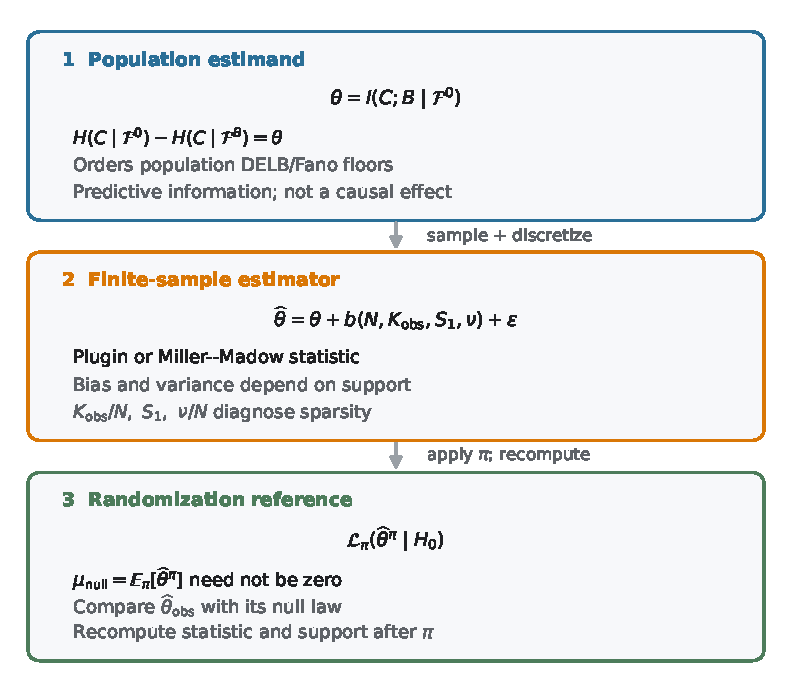
\includegraphics[width=0.92\textwidth]{figures/s7/e15_estimand_estimator_null_wide.pdf}
\caption{Population estimand, finite-sample estimator, and
transformation-specific randomization reference. CMI denotes predictive
information and is not interpreted as a causal effect.}
\label{fig:three_layers}
\end{figure}

\subsubsection{已知真值的稀疏嵌套状态模拟}
\label{subsec:e12_simulation_methods}

模拟在可完全枚举的概率模型下评估有限样本行为。基线状态 \(Z\) 具有
4、16 或 64 个类别，新增状态 \(B\) 具有 2、4 或 8 个类别，整数目标服从
条件负二项分布。因子设计交叉样本量 365 与 1095、均衡与偏斜状态概率、
零/中等/较强总体 CMI，以及独立或具有持续性的 Markov 状态序列。
总体 CMI 由精确求和得到，截断尾概率低于预设容差，而不是把大规模模拟
样本当作总体真值。

每个 216 个估计器设计单元生成 150 个样本，共得到 32,400 条重复记录。
plugin 与 Miller--Madow CMI 使用与经验分析相同的函数计算，并同时记录
\(K_{\mathrm{obs}}/N\)、\(S_1\) 和 \(\nu/N\)。第二个实验对总体零 CMI
与正 CMI 样本施加时间块、空间序列和循环位移变换。每个设计单元
包含 30 个 Monte Carlo 数据集，每个估计器和零设计使用 99 次变换。
因此，第一类错误率和功效只对应这些数据生成与变换机制，而不是所有 CMI
估计器或随机化方案。

\subsection{基于 DELB 的新增城市数据评价算法}
\label{subsec:delb_evaluation_algorithm}

\begin{Algorithm}[基于 DELB 的新增城市数据源评价]
\label{alg:delb_evaluation}
\textbf{输入：}整数目标 \(C\)、基准状态 \(\mathcal S^0\)、新增数据状态 \(B\)、
训练/验证/测试索引、熵估计器、随机化设计及重复次数 \(R\)。\\
\textbf{输出：}\(\widehat L^0\)、\(\widehat L^B\)、
\(\widehat{\Delta L}\)、\(\widehat I(C;B\mid\mathcal S^0)\)、支持度诊断、
随机化 \(p\) 值及匹配样本外预测误差。
\begin{enumerate}
    \item 仅使用训练期估计全部离散化阈值，并在验证与测试期固定。
    \item 在完全相同的合格观测上构造基准状态 \(\mathcal S^0\) 和增强状态
    \(\mathcal S^B=(\mathcal S^0,B)\)。
    \item 使用同一熵估计器计算 \(\widehat H(C\mid\mathcal S^0)\) 与
    \(\widehat H(C\mid\mathcal S^B)\)。
    \item 数值计算
    \(\widehat L^j=\mathcal H_{\mathbb Z}^{-1}
    [\widehat H(C\mid\mathcal S^j)]\)，其中 \(j\in\{0,B\}\)。
    \item 计算原始 CMI、DELB 估计的绝对和相对降幅，以及支持密度、
    singleton 占比和有效自由度诊断。
    \item 对每个预设随机化设计和每次重复，变换 \(B\)、重建
    \(\mathcal S^B\)，并重新计算状态支持及完整统计量；随后计算 plus-one
    上尾 \(p\) 值。
    \item 对每种预测模型使用相同样本、训练窗口、调参规则和全部非自行车输入
    进行两次拟合：一次使用 \(\mathcal S^0\)，一次使用 \(\mathcal S^B\)。
    \item 将 DELB 估计变化、随机化校准证据和测试集 MSE 变化作为三个独立
    输出比较。
\end{enumerate}
\end{Algorithm}

\paragraph{数值反演。}
对于正熵值，实现从 \(\lambda=1\) 开始反复减半或加倍以包围离散高斯率参数的根，
随后使用 Brent 方法求解。根容差为 \(10^{-12}\)，最多迭代 200 次。
当 \(\lambda\geq1\) 时，通过直接对称整数格点求和计算配分函数和二阶矩；
当 \(\lambda<1\) 时，使用 Poisson 对偶 theta 级数，避免在实格点上使用过宽
截断。两种情形均扩展支撑半径，直至遗漏双侧未归一化尾和的解析上界不超过
\(10^{-15}\)。小于或等于零的熵映射为零 DELB。重复重采样与随机化路径使用
配置的 0--8 bit 单调插值网格，并保留直接反演结果用于验证。

\paragraph{计算复杂度与并行。}
令 \(N\) 为匹配观测数，\(K_0\) 与 \(K_B\) 为两个状态表的非空原子数，
\(M\) 为格点求和保留的最大半支撑，\(T\leq200\) 为根函数计算次数，\(J\)
为需要转换为下界的熵值数量。状态计数需要 \(O(N)\) 时间和
\(O(K_0+K_B)\) 内存；直接下界转换需要 \(O(JTM)\) 时间及 \(O(M)\)
附加内存。使用 \(R\) 次随机化时，串行校准成本为
\(O(RN+RJTM)\)，不包括依赖具体预测器的模型拟合成本。在保存的随机种子
条件下，各随机化相互独立。多尺度实现使用 6 个线程并行处理独立的
城市--空间尺度--时间尺度单元，每完成一个单元即写入 checkpoint，同时保留
重复级输出和随机种子用于核对。


\subsection{城市与局部 DELB 估计}
\label{subsec:city_local_information}

城市层面 DELB 点估计在两个训练期冻结总体中评估，并按年份分别计算。完整
犯罪支持域表示预先规定的完整目标总体；自行车覆盖域表示能够观测新增移动
通道的服务覆盖总体。两个网格集合均由 2020--2021 年记录确定，随后不变地
用于验证与测试；任何 2022 年结果都不参与重新定义空间总体。因此，两者比较
针对目标分析总体，而不是行政边界。

使用 1000 次共享、互不重叠的七日历日块重抽样评价不确定性；重抽整个
城市--日块保留网格间同期依赖，报告 95\% 中心 bootstrap 区间。“共同主要”
总体的表述仅限城市层面点估计比较。局部估计、随机化校准、留出预测和多尺度
分析仍沿用各自预先规定的自行车覆盖域，因为这些实验并未全部生成完整域版本。

局部计算在每个网格内重复，并从局部状态中移除网格 ID。纳入标准为：
1095 个有效滞后日、至少 30 起犯罪、至少 55 个正流量日、零流量连续期不
超过 365 天，以及至少两个目标状态和两个自行车状态。最终得到
\TotalEligibleLocalGrids{} 个合格网格。基于七日块 bootstrap 的单侧
正态筛选采用 Benjamini--Hochberg 修正 \citep{benjamini1995}。
由于状态稀疏可能使熵差产生偏差，本文称其为“抽样不确定性筛选”，而不是
条件独立随机化检验。空间聚集使用行标准化 queen 邻接、999 次置换的全局
与局部 Moran 统计量 \citep{moran1950}。

\subsection{时空尺度与样本量三轴设计}
\label{subsec:e16_scale_methods}

为区分预测目标变化与估计稳定性变化，E16 从三个维度开展比较。空间分辨率为
500~m、1~km 和 2~km；时间分辨率为日和完整 ISO 周；样本比例为 20、40、
60、80 和 100\%。

比较域由完整的 2~km 父网格构成。每个父网格包含四个 1~km 子网格和十六个
500~m 后代网格，犯罪与自行车总量在该嵌套公共区域内严格守恒。周记录由七个
完整日求和，一期滞后始终表示前一聚合期。

样本比例通过选择时间块并保留其中全部网格形成。日面板使用完整七日块，周面板使用
完整四周块，并按年份和季节分层。五个比例在每个冻结重复内嵌套，20--80\%各有
50次重复；另以五个扩展窗口诊断按时间积累及潜在分布漂移。稳定性统计量定义为
\begin{equation}
S_N(\widehat\theta)
=\frac{|\widehat\theta_N-\widehat\theta_{N_{\max}}|}
{\max(|\widehat\theta_{N_{\max}}|,10^{-12})},
\label{eq:e16_stability}
\end{equation}
其中 \(\widehat\theta\) 表示熵、CMI 或 DELB 估计量。该指标衡量相对完整样本估计
的收敛，而不是相对未知总体真值的误差。

计数尺度 DELB 仍是主要 estimand。设正方形网格面积为 \(A\) km\(^2\)、聚合时长
为 \(\tau\) 日，则确定性缩放后的犯罪强度目标满足
\begin{equation}
L_{\mathrm{int,MSE}}^{j}(A,\tau)
=\frac{L^{j}(A,\tau)}{(A\tau)^2},
\qquad
L_{\mathrm{int,RMSE}}^{j}(A,\tau)
=\frac{\sqrt{L^{j}(A,\tau)}}{A\tau},
\quad j\in\{0,B\}.
\label{eq:e16_intensity_normalization}
\end{equation}
该换算仅适用于相应缩放的计数目标，并不会使日与周目标或不同空间聚合成为同一
estimand。本文不以样本量除 DELB 或 CMI。

随机化校准覆盖全部90个城市--空间--时间--样本单元。每个单元采用199次时间块、
空间序列及循环位移重复；预设的500~m--日、1~km--日和2~km--周关键尺度采用
999次。低于100\%的比例使用最低编号冻结稀释路径（重复1），稳定性分析另行汇总
全部50条稀释路径。时间块为七日或四周；循环位移至少相隔31日或五周。每次变换
后均重新计算Miller--Madow CMI、DELB下降、支持原子、singleton share和有效
自由度。plus-one上尾 \(p\) 值分别在全部270项及城市--零机制族内校正。这些是
设计条件诊断，而不是精确条件随机化检验。

\subsection{匹配预测与 Predictability Gap}
\label{subsec:prediction_experiment}
\label{subsec:methods_prediction}

式~\eqref{eq:empirical_baseline_state} 与
\eqref{eq:empirical_bicycle_state} 的成对状态下比较四类模型：
平滑状态均值、Poisson GLM、负二项 GLM，以及采用 Poisson 损失的直方图
梯度提升。每个模型族的基线与自行车增强规格使用相同目标、样本、预处理、
训练期、调参规则和整数后处理；增强规格仅加入
\(Q_B(B^{\mathrm{total}}_{t-1})\)。七日季节 naive 预测器仅作为外部
描述性基准，不与 DELB 状态匹配，也不进入主要比较。

超参数按验证期整数 MSE 选择。连续非负预测使用 half-up 规则转换为整数。
主要指标为
\begin{equation}
\operatorname{MSE}^{j}_{c,k}
=\frac{1}{N_c}\sum_{(i,t)\in\mathcal T_c}
\left(C_{c,i,t}-\widehat C^{\,j}_{c,i,t,k}\right)^2,
\quad j\in\{0,B\},
\label{eq:empirical_mse}
\end{equation}
其中 \(k\) 表示模型族，\(\mathcal T_c\) 是固定的 2022 年 7--12 月测试集。
正的
\(\Delta\operatorname{MSE}_{c,k}
=\operatorname{MSE}^{0}_{c,k}-\operatorname{MSE}^{B}_{c,k}\)
表示改善。1000 个共享且互不重叠的七日测试块保留网格间依赖；模型族筛选
使用单侧正态近似和 Benjamini--Hochberg 修正。

\subsection{次要 Fano、异质性与稳健性设计}
\label{subsec:fano_validation_methods}

固定有限标签目标用于补充整数计数 MSE 分析。主要目标为
\[
Y^{(2)}_{c,i,t}=\mathbf 1\{C_{c,i,t}>0\},
\]
稳健性目标将 \(C=0\)、\(C=1\) 和 \(C\geq2\) 映射为三类。
阈值全局预先固定，不由城市或测试结果选择。基线和自行车增强状态与
式~\eqref{eq:empirical_baseline_state} 和
\eqref{eq:empirical_bicycle_state} 完全相同。

条件熵与 Fano 下界在训练期加验证期上估计；随后在不变的
2022 年 7--12 月测试期评估逐状态众数分类器。2022 年 7 月前未见的测试
状态使用测试前总体众数回退，不使用任何测试标签设定回退规则。不确定性由
300 次互不重叠的七日历日块 bootstrap 得到。由于无条件重抽样本身可能
删除稀有状态，报告中心区间，同时保留原始 bootstrap 均值用于诊断。

oracle 检查复用可枚举概率模型，对二元和三级目标比较真实 Bayes
误差与真实 Fano 下界。经验比较则是估计测试前下界与留出分类器误差。
若出现估计违反，仍作为有限样本或分布漂移诊断保留。DELB 与 Fano 的
目标和损失不同，因此从不直接比较其数值。

\subsubsection{Predictability Gap 与理论--实践比较}
\label{subsec:gap_methods}
\label{subsec:gap_efficiency}

模型特定的预测差距为
\begin{equation}
G^j_{c,k}=\operatorname{MSE}^{j}_{c,k}-L^j_c
\label{eq:empirical_gap}
\end{equation}
及其收窄量
\begin{equation}
\Delta G_{c,k}
=G^0_{c,k}-G^B_{c,k}
=\Delta\operatorname{MSE}_{c,k}-\Delta L_c.
\label{eq:empirical_gap_narrowing}
\end{equation}
总体记号下，同一核算量为
\begin{equation}
G=\operatorname{MSE}-L,
\label{eq:prediction_gap}
\end{equation}
仅当分母为正时才可报告信息利用比率
\begin{equation}
\eta=\frac{\Delta\operatorname{MSE}}{\Delta L}.
\label{eq:bound_efficiency}
\end{equation}
正的 \(\Delta G\) 表示经验误差下降超过估计误差底线；负值表示理论机会
扩张快于所检验模型的利用速度。测试比较中的精确界在匹配测试窗口信息状态上
重新估计。

在局部尺度，将训练加验证期的测试前 \(\Delta L_{c,i}\) 与测试期
\(\Delta\operatorname{MSE}_{c,i,k}\) 比较。Spearman 相关使用 2000 次
成对网格 bootstrap 并进行 FDR 修正。另以城市固定效应和 HC3 标准误的
普通最小二乘模型回归局部经验改善对局部理论下降。该分析是描述性的，
回归协方差未建模跨网格依赖。

\subsubsection{犯罪类型异质性}
\label{subsec:crime_type_methods}

针对财产盗窃、机动车盗窃和入室盗窃重复信息与匹配预测分析，
使用分类别滞后计数，但保持自行车阈值和时间切分不变。共生成 18 个
城市--类别理论估计（合并期与测试期）、36 个成对测试预测对比，以及
城市内成对类别比较。七日块重抽样和 Benjamini--Hochberg 修正与主实验一致。

\subsubsection{替代设定与零分布校准}
\label{subsec:robustness_null_methods}

预设稳健性分析检查估计 DELB 下降的符号是否在设计改变下保持稳定。
16 个理论规格包括 500~m、1~km 和 2~km 网格；日与周目标；替代犯罪和
自行车状态映射；最多七日的犯罪与自行车滞后；以及流入、流出和绝对净流量。
每个规格采用 plugin、Miller--Madow 和一致的 Jeffreys--Dirichlet 估计器。
后者在 \((C_t,\mathcal S^0_t,B_{t-1})\) 的观测原子上放置单个对称
Dirichlet 后验，并通过边际聚合该后验得到两个条件熵。bootstrap 区间分别
使用 7、14 和 28 日块重新计算。预测稳定性在 2022 年 12 个扩展月度起点上
评估，每个起点使用一个月评估窗口和与主要匹配预测相同的四类模型。

三种诊断检验观测 CMI 是否超过有限样本参考分布。时间块置换重新分配七日
移动块，空间序列置换在网格间重新分配完整移动历史，循环位移替代则将每个
网格的移动序列移动一个合法随机偏移。每个设计使用 999 次变换、上尾
随机化 \(p\) 值和 Benjamini--Hochberg 修正。同样设计也应用于 339 个
合格网格。只有同时通过三个调整后检验的局部网格才被认定为通过
零分布校准。最后，将匹配的 14 日和 30 日滞后与近期一日滞后比较。
这些程序是诊断性随机化检验，不是精确条件随机化检验，也不是自行车因果
效应检验。

E17 检验城市层面校准结论是否依赖主要 Miller--Madow 修正。它在完全相同的
E10 替代样本上重新计算 plugin、Miller--Madow 和一致的 observed-support
Jeffreys--Dirichlet CMI。plus-one 上尾 \(p\) 值使用两类预设校正：
每个估计器内部九个城市--设计比较，以及全部 27 个估计器--城市--设计比较。
E17 不重跑 339 个局部网格筛查。Jeffreys 计算仅正则化观测到的完整联合原子
概率，并不填补未观测支持。

E18 在城市层面增加基准状态匹配的受限随机化。每个网格序列切分为完整七日块；
先按滞后犯罪状态分布与假日占用排序，再在同一网格、年份和季节内无放回置换，
不足五块的层在同一年内扩大，终端不完整块保持固定。设计使用 999 次随机化、
plus-one 上尾 \(p\) 值及三城市 Benjamini--Hochberg 修正。预设诊断要求
可移动块不少于 80\%，自行车状态边际的绝对标准化差不超过 0.10。

半合成实验在固定经验状态支持上评价校准与功效。每城确定性选择覆盖流量分位的
六个网格和 365 日。零机制下，负二项目标仅依赖经收缩估计的基准状态；随后通过
枚举校准中心化自行车状态效应，目标总体 CMI 为 0、0.02、0.05 和 0.10 bit，
但受各经验支持的最大可达值限制。因子设计交叉三个城市、拟合与增强过度离散
情景，以及原时间块和受限匹配块两种参考。每个单元使用 50 个 Monte Carlo
数据集及 99 次随机化，第一类错误率和功效同时报告精确二项式 95\% 区间。
该设计比 E10 更接近基准状态，但因其并非从已知
\(B\mid\mathcal S^0\) 分布抽样，仍不是精确条件随机化检验。

\subsubsection{替代样本特异支持度诊断}
\label{subsec:e13_support_methods}

每个已接受替代样本均按原始随机种子重建，并在每次变换后
重新计算 CMI 与状态支持度。对每个观测或随机化样本，记录
\begin{equation}
K_{\mathrm{obs}}
=\#\{(C,Z,B)\text{ observed atoms}\},
\qquad
S_1
=\frac{\#\{\text{observations in singleton atoms}\}}{N},
\label{eq:e13_support_metrics}
\end{equation}
以及
\begin{equation}
\nu=\sum_z(r_z-1)(c_z-1),
\label{eq:e13_effective_df}
\end{equation}
其中 \(r_z\) 与 \(c_z\) 是基线状态 \(z\) 内观测目标与自行车状态的
基数。分析使用 \(K_{\mathrm{obs}}/N\)、\(S_1\) 与 \(\nu/N\)。

模拟真值分析联系零分布偏差与支持度指标。经验关联以
Spearman 相关以及包含城市与零设计固定效应、城市--网格聚类标准误的回归
描述。模型把零分布均值联系到替代样本平均支持度，并把观测减零均值 CMI
联系到替代减观测支持度变化。这些关联用于诊断有限支持机制，但不会把
零均值变成估计器偏差估计，也不识别因果效应。

\subsection{可复现性与分析范围}
\label{subsec:reproducibility}

每个实验均由版本化 YAML 配置和 Python 命令行入口执行。运行目录包含
环境快照、随机种子、源运行指针、行数对账、验收检查、机器可读表格、
诊断工作簿和图片。所有论文图片均由对应 Python 实验生成，未进行手工编辑。
E11 只读取已接受 E02 与 E04--E10 输出；S7 Python 合成只读取已接受
E12--E15 输出，并把哈希核验的图片集复制到论文。E09 与 E10 在查看输出前
冻结；E12--E14 保存重复级模拟、支持度和 bootstrap 记录；E15 保存单栏与
双栏矢量概念图。所有正式输出均保留在版本化运行谱系中。
E16同样只读取已接受的多尺度面板、样本索引、估计与随机化结果；S16.7 Python
合成生成LaTeX宏和表格，并在SHA-256核验后复制全部尺度图。最小已知真值示例
\texttt{examples/minimal\_delb\_cmi\_simulation.py}无需城市数据即可复现总体CMI
排序和精确DELB数值逆；该示例仅用于教学，不替代注册的E12完整模拟网格。
